\documentclass[11pt]{article}

\usepackage{CMPSC465}
\usepackage{enumitem}
\usepackage{algpseudocode}
\usepackage{tikz}
\usepackage{tabularx}
\usepackage{amsmath}
\usepackage{tikz}
\usepackage{graphicx}
\usepackage[colorlinks=true, allcolors=blue]{hyperref}
\usepackage{tkz-graph}
\PassOptionsToPackage{usenames,dvipsnames,svgnames}{xcolor}  
\usepackage{tikz}
\usetikzlibrary{arrows,positioning,automata}
\def\title{Solution 07}

\def\defeq{\mathrel{\mathop:}=}
%\usepackage{algpseudocode}
%\usepackage{algorithm}
%\usepackage[ruled]{algorithm2e}
%\usepackage{amsthm}


\def\defeq{\mathrel{\mathop:}=}
%\usepackage{algpseudocode}
%\usepackage{algorithm}
\usepackage[ruled,noline]{algorithm2e}
%\usepackage{amsthm}
\newcommand\nonl{%
  \renewcommand{\nl}{\let\nl\oldnl}}% Remove line number for one line
  
\newcommand{\aaa}[1]{\hspace{0.65cm}\parbox[t]{15.3cm}{#1}}
\newcommand{\aab}[1]{\hspace{1.15cm}\parbox[t]{15.0cm}{#1}}
\newcommand{\aac}[1]{\hspace{1.65cm}\parbox[t]{15.0cm}{#1}}
\newcommand{\aad}[1]{\hspace{2.15cm}\parbox[t]{15.0cm}{#1}}
\newcommand{\aaA}[2]{\hspace{0.5cm} {\tikz[overlay] \draw (0.1, -0.1) -- (0.1, #1 * -1.5em + 0.6em);} \parbox[t]{15.0cm}{#2}}
\newcommand{\aaB}[2]{\hspace{1.0cm} {\tikz[overlay] \draw (0.1, -0.1) -- (0.1, #1 * -1.5em + 0.6em);} \parbox[t]{15.0cm}{#2}}
\newcommand{\aaC}[2]{\hspace{1.5cm} {\tikz[overlay] \draw (0.1, -0.1) -- (0.1, #1 * -1.5em + 0.6em);} \parbox[t]{15.0cm}{#2}}
\newcommand{\aaD}[2]{\hspace{2.0cm} {\tikz[overlay] \draw (0.1, -0.1) -- (0.1, #1 * -1.5em + 0.6em);} \parbox[t]{15.0cm}{#2}}
\newcommand{\xxx}{\par\vspace{0.1cm}}
\usepackage{tikz}

\begin{document}
\maketitle



\begin{qunlist}

\q{8}{} Run Dijkstra’s algorithm on the following graph, starting at node $A$. 
Whenever there is a choice of vertices with same $dist$ value, always pick the one that is alphabetically first. 
Specifically, you are asked to draw a table in which each row shows the $dist$ array at each iteration of the algorithm.

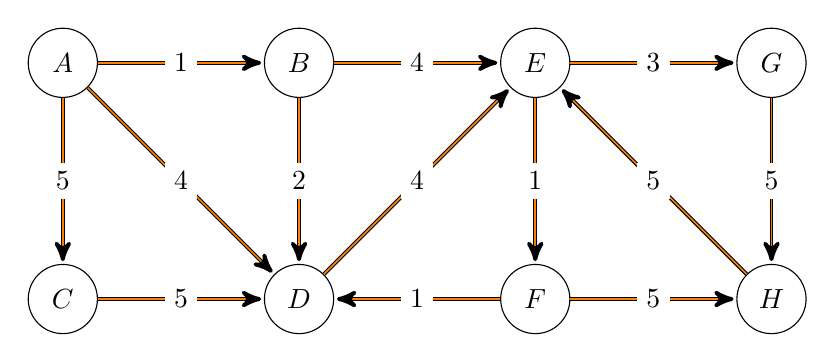
\begin{tikzpicture}[>=stealth',shorten >=1pt,node distance=3cm,on grid,initial/.style    ={}]
  \node[state]          (A)                        {$A$};
  \node[state]          (B) [right =of A]    {$B$};
  \node[state]          (C) [below =of A]    {$C$};
  \node[state]          (D) [below =of B]    {$D$};
  \node[state]          (E) [right =of B]    {$E$};
  \node[state]          (F) [below =of E]    {$F$};
  \node[state]          (G) [right =of E]    {$G$};
  \node[state]          (H) [right =of F]    {$H$};

\tikzset{mystyle/.style={->,double=orange}} 
\tikzset{every node/.style={fill=white}} 
\path (A)     edge [mystyle]    node   {$1$} (B)
      (A)     edge [mystyle]    node   {$5$} (C)
      (A)     edge [mystyle]    node   {$4$} (D)
      (B)     edge [mystyle]    node   {$2$} (D)
      (B)     edge [mystyle]    node   {$4$} (E)
      (D)     edge [mystyle]   node   {$4$} (E)
      (C)     edge [mystyle]   node   {$5$} (D) 
      (E)     edge [mystyle]   node   {$3$} (G)
      (E)     edge [mystyle]   node   {$1$} (F)
      (F)     edge [mystyle]   node   {$5$} (H)
      (F)     edge [mystyle]   node   {$1$} (D)
      (G)     edge [mystyle]   node   {$5$} (H)
      (H)     edge [mystyle]   node   {$5$} (E);

\end{tikzpicture}\\

\textbf{Solution:} Lets run the Dijkstra's algorithm on the given graph G(V,E)

\begin{tabularx}{0.5\textwidth} 
{ 
  | >{\raggedright\arraybackslash}X 
  | >{\centering\arraybackslash}X
  | >{\centering\arraybackslash}X
  | >{\centering\arraybackslash}X
  | >{\centering\arraybackslash}X
  | >{\centering\arraybackslash}X
  | >{\centering\arraybackslash}X
  | >{\centering\arraybackslash}X
  | >{\raggedleft\arraybackslash}X | 
}
 \hline
 Itr & A & B & C & D & E & F & G & H \\
 \hline
 0  & 0  & $\infty$  & $\infty$  & $\infty$  & $\infty$  & $\infty$  & $\infty$  & $\infty$  \\
 1  & \textbf{0}  & 1  & 5  & 4  & $\infty$  & $\infty$  & $\infty$  & $\infty$  \\
 2  & \textbf{0}  & \textbf{1}  & 5  & 3  & 5  & $\infty$  & $\infty$  & $\infty$  \\
 3  & \textbf{0}  & \textbf{1}  & 5  & \textbf{3}  & 5  & $\infty$  & $\infty$  & $\infty$  \\
 4  & \textbf{0}  & \textbf{1}  & \textbf{5}  & \textbf{3}  & 5  & $\infty$  & $\infty$  & $\infty$  \\
 5  & \textbf{0}  & \textbf{1}  & \textbf{5}  & \textbf{3}  & \textbf{5}  & 6  & 8  & $\infty$  \\
 6  & \textbf{0}  & \textbf{1}  & \textbf{5}  & \textbf{3}  & \textbf{5}  & \textbf{6}  & 8  & 11  \\
 7  & \textbf{0}  & \textbf{1}  & \textbf{5}  & \textbf{3}  & \textbf{5}  & \textbf{6}  & \textbf{8}  & 11  \\
 8  & \textbf{0}  & \textbf{1}  & \textbf{5}  & \textbf{3}  & \textbf{5}  & \textbf{6}  & \textbf{8}  & \textbf{11} \\
\hline
\end{tabularx}

\q{10}{}
There is a country of $n$ islands. $m$ bridges are installed between some of
these islands allowing us to travel in both directions.  We have two factories
on distinct islands and need to transport goods between theses two factories.
However, since each bridge has a weight limit, if an amount of goods exceeding
the weight limit passes though the bridge, the bridge will collapse. We know
that the weight limit of each bridge is at most $w$; you may assume that $w$ is an integer.
Design an algorithm to
find the maximum weight of the goods that can be moved in one transportation.
The time complexity of your algorithm should be $O((n + m) \log w)$. You can
get partial credits if you design an algorithm of $O((n + m)w)$.

\textbf{Solution: }
We can build a graph using islands as vertices and bridges as edges.
Suppose two factories are in islands A and B, we will load goods in the factory on island A and then move them to the one on island B. 
Let $M$ be the maximum weight of the goods can be moved from A to B in one transportation.
We know there are $w+1$ possible number of maximum weight $\{0,1,2,...w\}$. %(e.g., 0 means there is no path from A to B, 5 means $M$ is 5).
We can use binary search to find $M$. For a particular maximum-weight $mid$, we can test whether there exists a path from A to B on which all edges have limit at least $mid$~(i.e., goods of weight $mid$ can be transported from A to B) by first removing all edges whose weight limit is below $mid$ and then testing if A can reach B in the resulting graph using BFS or DFS.

Step 1: construct the graph $G$ using islands as vertices and bridges as edges.\\
Step 2: initialize four integers, $low = 0, high = w, mid = 0, max\_w = 0$.\\
Step 3: update $mid$, $mid = (low+high)/2$; make a copy of $G$ and name it as $G'$; then update the adjacency list of $G'$ to remove any edge whose weight is less than $mid$.\\
Step 4: run BFS/DFS to find if there is a path from A to B in $G'$. If yes, it means $M$ is at least $mid$, so we have $max\_w = mid$ and $low = mid+1$; otherwise, it means $M$ is less than $mid$, so we have $high = mid-1$.\\
step 5: while $low \leq high$, repeat steps 3--4. Return $max\_w$ after finishing the while loop.

Running time: time complexity of step 1 is $O(n+m)$, time complexity of step 2 is $O(1)$, time complexity of step 3 is $O(m)$, time complexity of step 4 is $O(n+m)$. We may need to run multiple times of step 3 and step 4, and the number of times is $O(\log w)$ since we are doing binary search and in each iteration $(high-low)$ will be halved. So the total running time is $O((n + m) \log w)$.


\q{10}{}
For a given directed graph $G = (V, E)$, let us denote $V = \{1, 2, ..., n\}$.
Define a function $D(G, s, t)$ that gives the distance from $s$ to $t$.
%using Dijkstra's algorithm. %Suppose we now are interested in a shortest path from $1$ to $n$.

\begin{enumerate}
    \item We want to get the length of the shortest path from $1$ to $n$ that must pass through a vertex $v$. 
	Prove that $D(G, 1, v) + D(G, v, n)$ gives the desired quantity. You may use proof by contradiction.
    \item We want to get the length of the shortest path from $1$ to $n$ that must pass through two vertices $v$ and $w$. 
	Using the above, find a formula to represent the quantity in terms of the function $D$ and vertices $1, n, v, w$.
\end{enumerate}
\textbf{Solution: }
\begin{enumerate}
    \item 
    Suppose that there exists a path $p$ from 1 to $n$ passing through $v$ with distance $d < D(G, 1, v) + D(G, v, n)$. We can divide $p$ into two parts $p_1$ and $p_2$ so that $p_1$ is a path from 1 to $v$ and $p_2$ is a path from $v$ to $n$. Let $d_1$ and $d_2$ be the distance from 1 to $v$ via $p_1$ and from $v$ to $n$ via $p_2$, respectively. Then, $d = d_1 + d_2 <  D(G, 1, v) + D(G, v, n)$. If $d_1 < D(G, 1, v)$, it is a contradiction because $D(G, 1, v)$ returns the shortest path from 1 to $v$ so it must count $p_1$ during the function as well. Therefore, $d_1 \geq D(G,1,v)$. Similar to this, we also obtain that $d_2 \geq D(G,v,n)$. Combining these two inequalities gives us $d_1 + d_2 \geq D(G,1,v) + D(G, v, n)$, which is a contradiction. Therefore, there is no path from 1 to $n$ passing through $v$ with a shorter distance than $ D(G, 1, v) + D(G, v, n)$\\
    We also need to make sure that $D(G, 1, v) + D(G, v, n)$ is indeed the shortest path from $1$ to $n$ passing through a vertex $v$. $D(G, 1, v)$ returns the shortest path from 1 to $v$, so we can make sure that there exists a path $p_1$ from 1 to $v$ with the distance $D(G, 1, v)$. The same goes for the case of $v$ and $n$, denote it as $p_2$. Then, by concatenating $p_1$ and $p_2$, we obtain the desired path with distance $D(G, 1, v) + D(G, v, n)$.
    \item If we must pass two vertices $v$ and $w$, there are two possible paths of $1 \rightarrow v \rightarrow w \rightarrow n$ and $1 \rightarrow w \rightarrow v \rightarrow n$. Using the above, we figure out that the corresponding shortest paths are $D(G,1,v) + D(G, v, w) + D(G, w, n)$ and $D(G,1,w) + D(G, w, v) + D(G, v, n)$, respectively. Therefore, we can obtain the desired shortest path by $\min\{D(G,1,v) + D(G, v, w) + D(G, w, n), D(G,1,w) + D(G, w, v) + D(G, v, n)\}$
\end{enumerate}

\q{8}{} You are given a directed graph $G = (V,E)$ and a vertex $s\in V$. Each edge $e$ is assigned with a length $l(e)$, possibly with negative value. We know that there is no negative cycle in this graph, and that the only negative edges are the ones that leave the vertex $s$. That is, $l(s, v) < 0$ for all $(s, v) \in E$, and $l(u,v) > 0$ for all $u\neq s$ and $(u,v)\in E$. If we run Dijkstra’s algorithm starting at $s$, will it fail on this graph? Prove your conclusion.\\
\textbf{Solution: } No, it won't fail on this graph.\\
Proof: The correctness of Dijkstra's algorithm depends on the claim that the next closes vertex, i.e., $v^*_{k+1}$, must be within one-edge extension of $R_k$ i.e. $v^*_{k+1} = \arg\min_{v\not\in R_k, u\in R_k, (u,v)\in E} (distance(s,u) + l(u,v))$. The proof of this statement \emph{only} uses that, the edges \emph{leaving} any $v\not\in R_k$ have positive edge length. In other words, the proof \emph{only} requires that the one-edge extension is always preferred than the two-edge extension~(first edge being $(u,v)$, second edge being $(v,w)$ for some $w$) will always be longer since the second-edge has positive edge length. In our case, the second-edge always has positive length. This is because, although edges leaving $s$ have negative edge length, $s$ will always stay in $R_k$ and consequently edges leaving $s$ will always be part of one-edge extension. 
%We can follow the same proof in the lecture note because although edges leaving $s$ have negative length, we still have $l(w, v^*_{k+1}) > 0$ and consequently $dist(s, w) < dist(s, v^*_{k+1})$, which are the keys of the proof. The only thing affected is that $dist(s, w)$ could be negative, but the proof doesn't need it to be non-negative.

\newpage
{\huge {\bf Rubrics:}}

\bigskip

    
{\bf Problem 1, 8pts}
\begin{enumerate}
    \item 8 pts : All the iterations and final answer are correct
    \item 6 pts : Didn't follow alphabetical order(i.e., the final answer is correct the choice of vertices in the iterations are different).
    \item 3 pts : more than half of the final shortest paths(>4) are correct.
    \item 0.8 pt : I don't know how to answer this question.
\end{enumerate}

{\bf Problem 2, 10pts}
\begin{enumerate}
    \item 
    \begin{itemize}
        \item 10pts : correct algorithm with $O((n + m) \log w)$ running time.
        \item 7pts : correct algorithm with $O((n + m) w)$ running time.
        \item 5pts : incorrect algorithm but apply path finding algorithms (BFS/DFS).
    \end{itemize}
    1pt : I don't know how to answer this question.
\end{enumerate}

{\bf Problem 3, 10pts}
\begin{enumerate}
    \item 
    \begin{itemize}
        \item 3pts : Proved there is no desired path with a shorter distance than $D(G, 1, v) + D(G, v, n)$.
        \item 3pts : Proved $D(G, 1, v) + D(G, v, n)$ is indeed the desired shortest path.
    \end{itemize}
    \item
    \begin{itemize}
        \item 4pts : Provided a correct formula.
        \item 2pts : Provided one of them.
    \end{itemize}
    
    1pt : I don't know how to answer this question.
\end{enumerate}

{\bf Problem 4, 8pts}
\begin{itemize}
    \item 3pts: Correct conclusion.
    \item 5pts: Provided a proof that makes sense.
    \item 0.8pts: I don't know how to answer this question.
\end{itemize}

\end{qunlist}
\end{document}
